\documentclass[xcolor=dvipsnames]{beamer}

\usepackage[english]{babel}
\usepackage{csquotes}
\usepackage{multicol}
\usepackage{amsmath}
\usepackage{amssymb}
\usepackage[style=authortitle, backend=biber]{biblatex}
\DefineBibliographyStrings{ngerman}{andothers = {{et\,al\adddot}},}
\addbibresource{lit.bib}

\usetheme{Madrid} 
\useinnertheme{rectangles}
\setbeamertemplate{navigation symbols}{}
\setbeamertemplate{blocks}[default]
\setbeamerfont{section number projected}{size=\large}
\setbeamertemplate{frametitle continuation}[from second][]
\setbeamercovered{transparent=15}
\setbeamertemplate{caption}[numbered]

\definecolor{cadet}{rgb}{0.33, 0.41, 0.47}   

\setbeamercolor{section in toc}{fg=black}
%\setbeamercolor{block title}{bg=yellow, fg=white}
\setbeamercolor{palette primary}{bg=cadet,fg=white}
\setbeamercolor{palette secondary}{bg=cadet,fg=white}
\setbeamercolor{palette tertiary}{bg=cadet,fg=white}
\setbeamercolor{structure}{fg=cadet} 

%https://tex.stackexchange.com/questions/68080/beamer-bibliography-icon
\setbeamertemplate{bibliography item}{%
  \ifboolexpr{ test {\ifentrytype{book}} or test {\ifentrytype{mvbook}}
    or test {\ifentrytype{collection}} or test {\ifentrytype{mvcollection}}
    or test {\ifentrytype{reference}} or test {\ifentrytype{mvreference}} }
    {\setbeamertemplate{bibliography item}[book]}
    {\ifentrytype{online}
       {\setbeamertemplate{bibliography item}[online]}
       {\setbeamertemplate{bibliography item}[article]}}%
  \usebeamertemplate{bibliography item}}

\defbibenvironment{bibliography}
  {\list{}
     {\settowidth{\labelwidth}{\usebeamertemplate{bibliography item}}%
      \setlength{\leftmargin}{\labelwidth}%
      \setlength{\labelsep}{\biblabelsep}%
      \addtolength{\leftmargin}{\labelsep}%
      \setlength{\itemsep}{\bibitemsep}%
      \setlength{\parsep}{\bibparsep}}}
  {\endlist}
  {\item}

% a nice alternative: https://tex.stackexchange.com/questions/178800/creating-sections-each-with-title-pages-in-beamers-slides
\AtBeginSection[]
{
    \begin{frame}
        \frametitle{Overview}
        \setbeamertemplate{section in toc}[square]
        \tableofcontents[currentsection]
    \end{frame}
}

\title[alt title]{Deep Learning Methods \\ for Financial Sentiment Analysis}
\date{}
\author[alt author]{Jimmy Neutron}
\institute[alt institution]{University of Narnia}

\begin{document}

\maketitle

\begin{frame}{Overview}
\setbeamertemplate{section in toc}[square]
\tableofcontents
\end{frame}

\section{ML Basics}

\begin{frame}[t]{A.I.}{A nice slide subtitle} \vspace{5pt}
\begin{block}{Definition}
this is a definition 
\end{block}
\begin{exampleblock}{Example} 
this is an example 
\end{exampleblock}
\begin{alertblock}{Alert}
this is an alert!
\end{alertblock}
\end{frame}

\begin{frame}[t]{Supervised Learning}\vspace{5pt}
Consider a set of labeled examples: $ \{ (x_i, y_i) \} ^N_{i=1}$. Each example is represented by a unique vector $x_i \in \mathbb{R}^D $ and each dimension  $x^{(j)}$ $(j = 1, ..., D)$ represents a certain feature.
\end{frame}

\begin{frame}[t]{Title}{A nice slide subtitle}\vspace{5pt}
Take a look at the following equations:
\begin{equation}
    \hat{\sigma}^2 = \frac{1}{n-1}\sum^n_{i=1}(x_i - \bar{x})^2
\end{equation}
\begin{equation}
    \overline{x} = \frac{1}{n}\sum^n_{i=1}x_i
\end{equation}
\end{frame}

\section{Stuff}

\begin{frame}[t]{List}\vspace{5pt}
Here is an unnumbered list:
\begin{itemize}
    \item this
    \item is
    \item a test
\end{itemize}
And here is one with numbers:
\begin{enumerate}
    \item :-)
    \item :-C 
    \item =(O.O)=
\end{enumerate}
\end{frame}

\begin{frame}[t]{Table}\vspace{5pt}
\begin{table}[]
\begin{tabular}{|lllll|}
\hline
A & B  & C  & D  & E  \\ \hline
1 & 2  & 3  & 4  & 5  \\
2 & 4  & 6  & 8  & 10 \\
5 & 10 & 15 & 20 & 25 \\ \hline
\end{tabular}
\caption{My Table}
\end{table}
\end{frame}

\begin{frame}{Table}\vspace{5pt}
\begin{table}[]
\begin{tabular}{|lllll|}
\hline
A & B  & C  & D  & E  \\ \hline
1 & 2  & 3  & 4  & 5  \\
2 & 4  & 6  & 8  & 10 \\
5 & 10 & 15 & 20 & 25 \\ \hline
\end{tabular}
\caption{My other Table}
\end{table}
\end{frame}

\section{More Stuff}

\begin{frame}[t]{Columns}\vspace{5pt}
\begin{multicols}{2}
text text text text text text text text text text text text text text text text text text text text text text text text text text \textcolor{RedOrange}{text} text text text \columnbreak text text text text text text text text text text text text text text text text text text text text text text text text text text text text text text text text \colorbox{Dandelion}{text} text text text text text text text text text text text text text text text text text text text text text  
\end{multicols}
\end{frame}

\begin{frame}{img}\vspace{5pt}
\begin{figure}
    \centering
    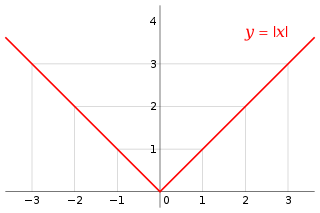
\includegraphics[scale=0.7]{img/320px-Absolute_value.svg.png}
    \caption{My Figure}
    \label{fig:my_label}
\end{figure}
\end{frame}

\begin{frame}[t]{citation}\vspace{5pt}
Text text \footcite{attention}
\end{frame}
 
\begin{frame}[t]{citation and footnote}
Text text \footcite{goodfellow} and more Text\footnote{Hello, this is a test.}
\end{frame}
 
\begin{frame}[b]{bottom}{A nice slide subtitle}\vspace{5pt}
\begin{center}
I am at the bottom of the slide
\end{center}
\end{frame}
 
\section{Another Section}
 
\begin{frame}{center}{A nice slide subtitle}\vspace{5pt}
center left \footcite{goldberg}
\end{frame}

\begin{frame}
\frametitle{A Theorem on Infinite Sets}
\begin{theorem}
There exists an infinite set.
\end{theorem}
\begin{proof}[testProof]
This follows from the axiom of infinity.
\end{proof}
\end{frame}
 
\begin{frame}{only command}
\only<1->{First Line of Text}

\only<2->{Second Line of Text}

\only<3>{Third Line of Text}
\end{frame}

\begin{frame}{onslide command, with transparency}
\begin{itemize}
    \item this
    \onslide<2->{
    \item is}
    \onslide<3->{
    \item a test}
\end{itemize}
\end{frame}

\begin{frame}[allowframebreaks]{Reference Slide Title}
\printbibliography[title=Reference Slide Title]
\end{frame} 

\end{document}
